\documentclass[Main.tex]{subfiles}

\usepackage{graphicx}

\begin{document}
The anchoring effect is explained on page xxx of Kahneman. 

The anchoring effect is measured in percentages by dividing the differences between averages by the difference between the anchors. For example. The difference between the anchors 3 and 9 is 6 and the difference between the averages 5 and 7 is 2. Then, the anchoring effect is 2/6, or 30\%. An anchoring effect of 100\% means the subjects adapts the anchor point and an anchoring effect of 0\% means the anchor has no effect on people. 

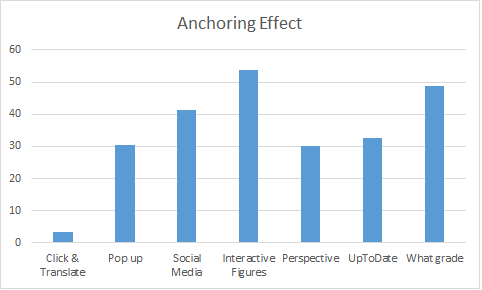
\includegraphics[width=\textwidth]{Anchoringpictures}

In the results we see that there was almost no anchoring affect on the question about the dictionary feature (only 3.5\%). This is probably because students already know the feature and like it. As we discussed before: if someone sees the anchor being very low but actually likes the feature very much they might anchor to a very high number because they think the low grade is very weird.

The question about the interactive figures had a very strong anchoring effect, it was 53\%. This is probably one of the examples that people in general do not have a high opinion of so they are easily influenced by the anchor.

Overall we can conclude the anchors did effect the answers to the questions in almost all of the questions. Therefore, no anchors should be put when doing an prototype session. If people do not have a very strong opinion about the prototype they might adjust towards the anchor and the results will not be entirely true.

\end{document}